\section{Filter\hartl{509}}

\begin{longtable}{|>{\bfseries}p{3cm}|c|p{10cm}|}
    \hline
    1. Ordnung
    & 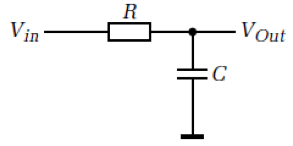
\includegraphics[width=4cm, valign=t]{pictures/tiefpass1ordnung}
    & {\textbf{UTF: } $G(s): \frac{1}{1+s C\cdot R} = \frac{1}{1+ j\cdot \frac{\omega}{\omega_{3dB}}}$\newline
        $f_{3dB}=\frac{1}{2\pi R\cdot C}$\newline
        Bei $\omega=\omega_{3dB}=\frac{1}{\tau}$ sind Real- und Imaginärteil gleich gross:
        
        $T=R \cdot C$
      }
    \\ \hline
% ----------------------------------------------------------------------------------------------------    
    {2. Ordnung\newline
     (kaskadierte RC-Tiefpässe)
    }
    & 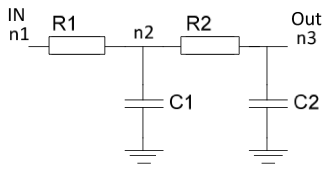
\includegraphics[width=6cm,angle=90, valign=t]{pictures/tiefpass2ordnung}
    & {$G(s) = \left(\frac{1}{1+sRC}\right)^2 = \left(\frac{1}{1+sT}\right)^2$ \newline
       $T = \frac{\sqrt{\sqrt{2}-1}}{2\pi \cdot f_g}$ \newline
       $G_{p}(s)= \frac{U_{out}}{U_{in}} = 
       \frac{1}{C_1\cdot C_2\cdot R_1\cdot R_2\cdot s^2+ (C_1\cdot R_1 + C_2\cdot R_1 + C_2\cdot R_2)\cdot s+1}$    
       \newline\newline
       \textbf{2.komplexe Pole:} \newline
       $G(s) = \frac{p_1 \cdot p_2}{(p_1+s)(p_2+s)}=\frac{\omega_0^2}{s^2+s\cdot\frac{\omega_0}{Q}+\omega_0^2}$ \newline
       \begin{tabular}{p{5cm}p{5cm}}
         $p_1 = \frac{\omega_0}{2Q}(1+\sqrt{1-4Q^2})$ &
         $p_1 = \frac{\omega_0}{2Q}(1-\sqrt{1-4Q^2})$
       \end{tabular}
       
       \textbf{Vgl. allgemeiner Tiefpass 2. Ordnung:}\newline
       \begin{align*}
           G_{LP}(s)	= \frac{A0}{\frac{s^2}{\omega_{0}^2}+\frac{s}{Q\cdot\omega_{0}}+1} &
           \quad A0 = 1 \\
           \omega_{0}	= \frac{1}{\sqrt{C_1\cdot C_2\cdot R_1\cdot R_2}}&\quad Q=\frac{\sqrt{C_1\cdot C_2\cdot R_1\cdot R_2}}{R_1\cdot (C_1+C_2)+C_2 \cdot R_2}
        \end{align*}
        } \\
        \textbf{Schrittantwort:}&{
        
        identische Pole: }&{
        \[y_{\sigma}(t) = 1-\e^{-\frac{t}{T}}\cdot(1+\frac{t}{T})\] }\\
          &{
        ungleiche Pole: }&{
        \[y_{\sigma}(t) = 1-\left(\frac{T_1 \cdot \e^{-\frac{t}{T_1}}- T_2 \cdot
        \e^{-\frac{t}{T_2}}}{T1-T_2}\right) \]}\\
        &{komplexe Pole:}&{
        \begin{align*}
          y_{\sigma}(t) = &1-\e^{-\frac{\omega_0}{2Q}\cdot t}\cdot \\
          &\left[\cos \left(\frac{\omega_0}{2Q} \sqrt{4Q^2-1} \cdot t \right) +
          \frac{1}{\sqrt{4Q^2-1}}\cdot \sin\left(\frac{\omega_0}{2Q} \sqrt{4Q^2-1} \cdot t \right)\right]
        \end{align*} \newline
        
        Passive RC-Filter können maximal Güte von 0.5 haben (2 identische reelle Pole) Filter höherer 
        Güte werden Spulen oder Verstärker benötigt. Für Systeme 2.Ordnung ist eine Polgüte von 0.7 optimal.
      }
      \\ \hline
      
      \end{longtable}
      
\begin{minipage}{0.49\textwidth}
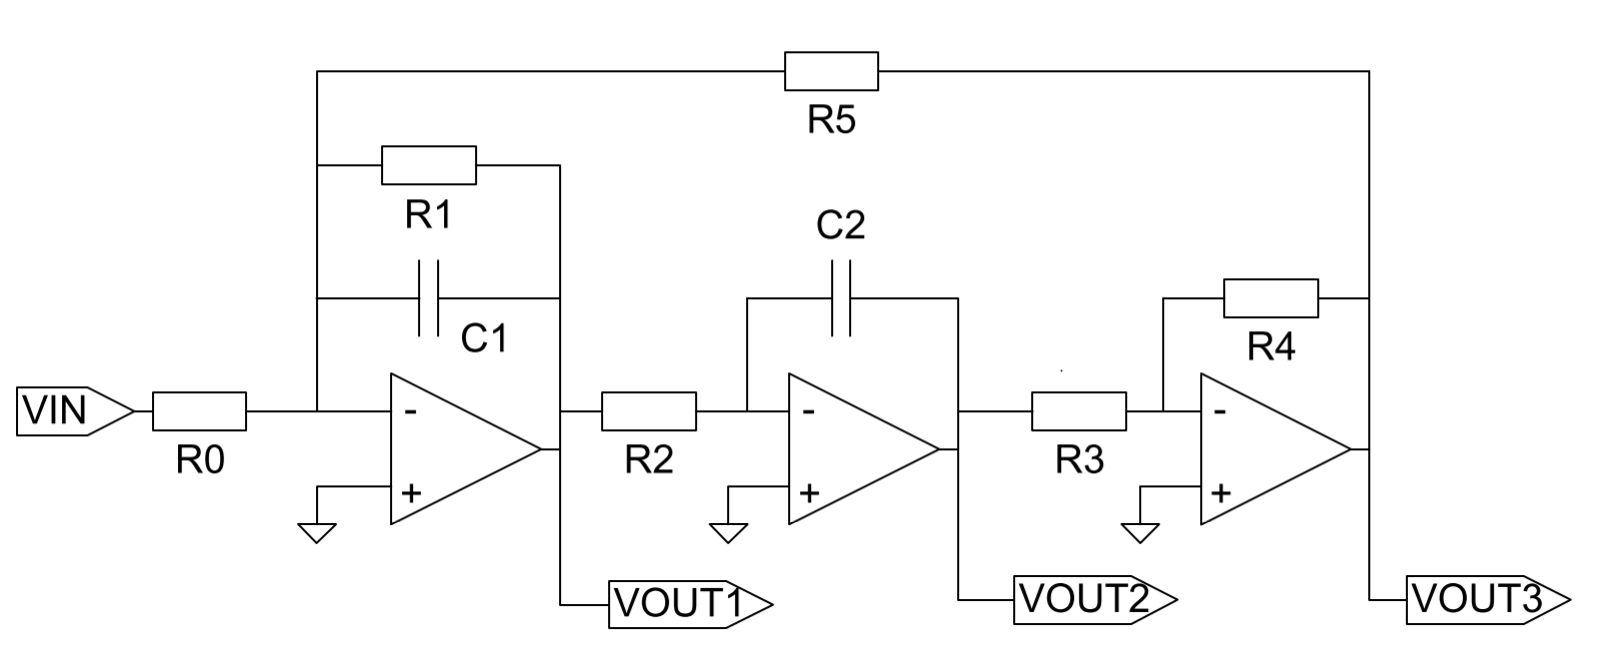
\includegraphics[width = 0.99\textwidth]{pictures/filter.png}
\end{minipage}
\begin{minipage}{0.49\textwidth}
$
G1i = V_{OUT1}(V_{IN})\quad G1f = V_{OUT1}(V_{OUT3})
$\\
$
G2 = V_{OUT2}(V_{OUT1}) \quad G3 = V_{OUT3}(V_{OUT2})
$\\[1em]
\begin{minipage}[t]{0.49\textwidth}
$
G1i = \dfrac{-R_1}{R_0\cdot(C_1\cdot R_1\cdot s+1)}
$\\
$
G2 = \dfrac{-1}{C_2\cdot R_2\cdot s}
$	
\end{minipage}
\begin{minipage}[t]{0.49\textwidth}
$
G1f = \dfrac{-R_1\cdot V_{OUT3}}{R_5\cdot(C_1\cdot R_1\cdot s+1)}
$\\
$
G3 = \dfrac{-R_4}{R_3}
$
\end{minipage}

\begin{minipage}[t]{0.39\textwidth}
Gesamtgain bestimmen mit Mason:
\end{minipage}\hfill
\begin{minipage}[t]{0.49\textwidth}
$
G_{13} = \dfrac{G1i\cdot G_2\cdot G_3}{1-G_{1f}\cdot G_2\cdot G_3}
$
\end{minipage}\\
\[
G = \dfrac{\frac{-R_1}{R_0\cdot(C_1\cdot R_1\cdot s+1)}\cdot \frac{-1}{C_2\cdot R_2\cdot s}\cdot \frac{-R_4}{R_3}}{1-\left(\frac{-R_1}{R_5\cdot(C_1\cdot R_1\cdot s+1)}\cdot 	\frac{-1}{C_2\cdot R_2\cdot s}\cdot \frac{-R_4}{R_3}\right)}
\]
\[
G = \frac{R_1\cdot R_4\cdot R_5}{R_0\cdot \left(C_1C_2R_1R_2R_3R_5 s^2 + C_2R_2R_3R_5 s + R_1R_4\right)}
\]
\end{minipage}

Vorgehen: 
\begin{enumerate}
\itemsep0em
\item Einzelne Übertragungsfunktionen aufstellen
\item Gesammtgain mittels Mason bestimmen
\item Kürzen
\item Wenn gefragt Gain bei DC und $\omega \rightarrow \infty$ bestimmen
\end{enumerate}
\pagebreak
\begin{longtable}{|>{\bfseries}p{3cm}|c|p{10cm}|}
\hline   \textbf{Kaskadierter Spannungsteiler}
      & %TODO Bild einfügen
      &
      \[
				H(s) = \frac{Y(s)}{X(s)} = \frac{Z_2 Z_4}{Z_1Z_2+Z_1Z_3+Z_1Z_4+Z_2Z_3+Z_2Z_4}      
      \]\\ \hline
%----------------------------------------------------------------------------------------------------      
    {Sallen Key\newline
     (Einfachmit-kopplung)\newline
     \hartl{517}
    }
    & 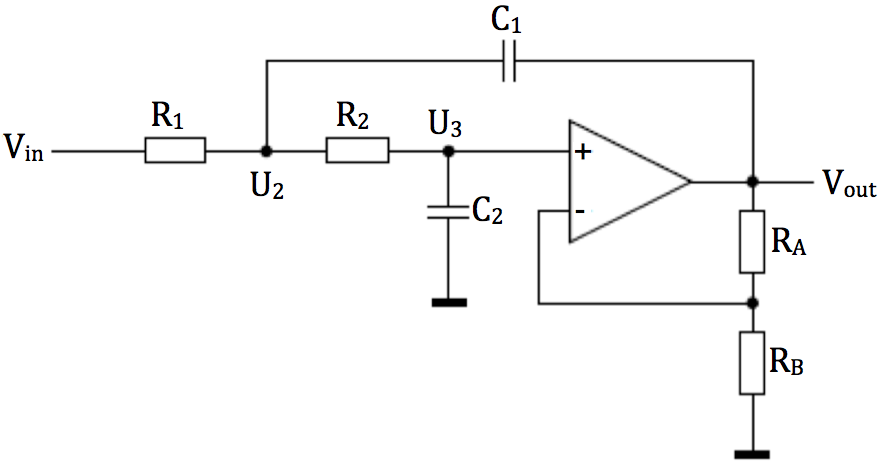
\includegraphics[width=6cm, angle = 270,valign=t]{./pictures/sallenkey.png}
    & {\textbf{ Standard Sallen Key}\newline
       Stromgleichungen:\newline
       $0 = (U_2-U_{in})\cdot \frac{1}{R_1}+(U_2-U_3)\cdot \frac{1}{R_2}+(U_2-U_{out})\cdot s C_1$ \newline
       $0 = (U_3-U_2)\cdot \frac{1}{R_2}+U_3\cdot s C_2$\newline
       Verstärkung:\newline
       $U_{out}=G_0\cdot U_3$ mit $G_0 = \frac{R_{A}+R_{B}}{R_{B}}$\newline
       \begin{align*}
           G_{SK}	&= \frac{G_0}{C_1\cdot C_2\cdot R_1\cdot R_2\cdot 
           s^2+[C_2\cdot (R_1+R_2)+C_1\cdot R_1\cdot (1-G_0)]\cdot s +1}\\
           \omega_0 &= \frac{1}{\sqrt{C_1\cdot C_2\cdot R_1\cdot R_2}}\\
           Q_{SK}	&= \frac{\sqrt{C_1\cdot C_2\cdot R_1\cdot R_2}}{C_2\cdot (R_1+R_2)+C_1\cdot R_1\cdot (1-G_0)}
       \end{align*}
      Die Güte kann mit $G_0$ beeinflusst werden. SK-Filter sind für grosse Güten nicht geeignet.
      }
    \\
    & 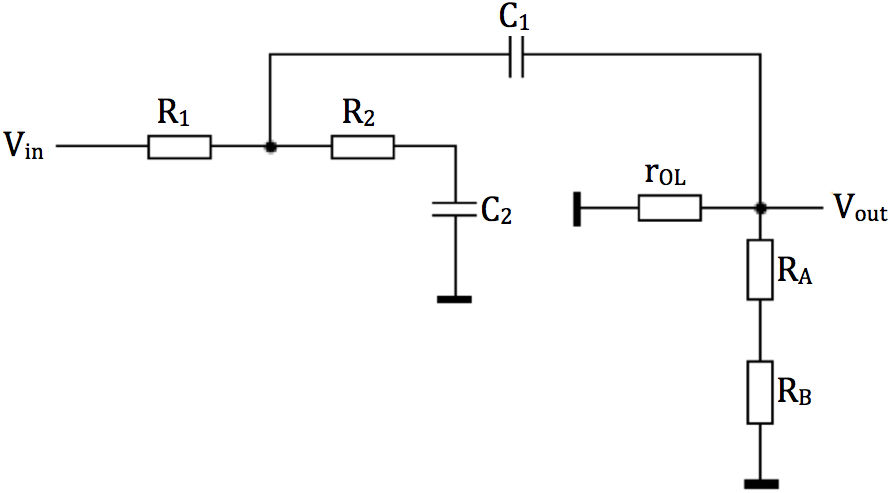
\includegraphics[width=4cm, valign=t]{./pictures/sallenkey2.png}
    & {\textbf{ für hohe Frequenzen}\newline
        \vspace{-1.5\topsep}
        \begin{itemize}[leftmargin=*]
            \item Wenn der Opamp nicht mehr verstärkt
            \item $C_1$, $C_2$ wirken als Kurzschlüsse
            \begin{equation*}
                \frac{V_{Out}}{V_{in}}=\frac{r_{OL}\parallel R_2\parallel
                    (R_{A}+R_{B})}{R_1+r_{OL}\parallel R_2\parallel (R_{A}+R_{B})}\approx
                \frac{r_{OL}}{R_1+r_{OL}}
            \end{equation*}
            \item Folge: Sallen Key-Filter sind nicht geeignet für Systeme mit hohen
            Frequenzanteilen, z.B. PWM-DAC
            \item $r_{OL}$: OpAmp OpenLoop Ausgangswiderstand
        \end{itemize}   
      }
      \\ \hline
% ---------------------------------------------------------------------------------------------------- 
      {Multiple Feedback\newline
       \hartl{522}
      }
      & 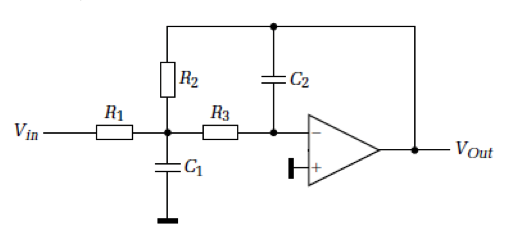
\includegraphics[width=4cm, valign=t]{./pictures/mulipleFeedback.png}
      & {Stromgleichungen: (Opamp sorgt für $U_3=0$)\newline
         $0	=(U_2-U_{in})\cdot \frac{1}{R_1}+(U_2-U_{out})\cdot \frac{1}{R_2}+(U_2-U_3)\cdot \frac{1}{R_3}+U_2\cdot s C_1$\newline
         $0	=(U_3-U_2)\cdot \frac{1}{R_3}+(U_3-U_{out})\cdot s C_2$\newline\newline
         $G_{mf}(s)	=\frac{G_0}{1+C_2(R_2+R_3+R_3\cdot \frac{R_2}{R_1})\cdot s+C_1\cdot C_2\cdot R_2\cdot R_3\cdot s^2}$ mit $ G_0 = -\frac{R_2}{R_1}$\newline
         $Q_{mf} =\frac{\sqrt{C_1\cdot C_2\cdot R_2\cdot R_3}}{C_2\cdot (R_2+R_3+R_3\cdot \frac{R_2}{R_1})}$ \qquad $\omega_0 = \frac{1}{\sqrt{C_1 \cdot C_2 \cdot R_2 \cdot R_3}}$\newline
         Die Güte wird v.a. eingestellt mit $C_2$ und $R_1$, grosse Güte für kleines $C_2$ und grosses $R_1$. $C_2$ beeinflusst auch das Frequenzverhalten, $R_1$ die Verstärkung.
        }
      \\ \hline
% ---------------------------------------------------------------------------------------------------- 
      {Zustandsvariab-len-Filter
      }
      & 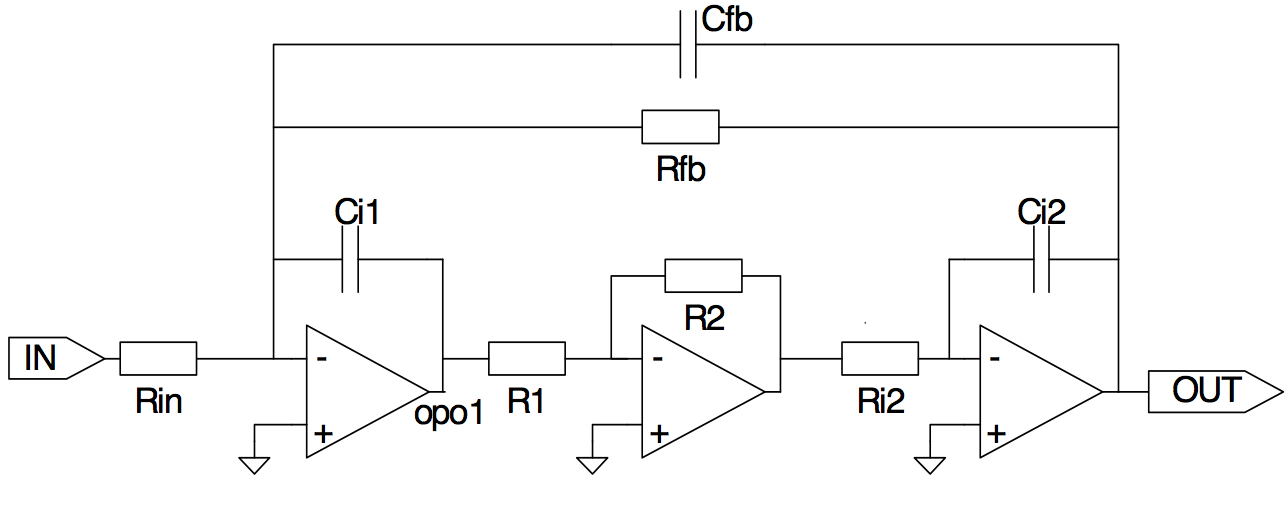
\includegraphics[width=8cm, valign=b,angle=270]{./pictures/zustandsvariable.png}
      & {Spannungsgleichungen:\newline
         \begin{align*}
             V{out}		&=-\frac{1}{s C_{i2}\cdot R_{i2}}\cdot V_{opo2}\\
             V_{opo2}	&=-\frac{R_2}{R_1}\cdot V_{opo1}\\
             V_{opo1}	&=\frac{-1}{s C_{i1}}\cdot \left(\frac{V_{in}}{R_{in}}+
             \frac{V_{out}}{R_{fb}}+s C_{fb}\cdot V_{out}\right)\\
             G_{ss}(s)	&=\frac{-\frac{R_{fb}}{R_{in}}}{C_{i1}\cdot C_{i2}\cdot R_{i2}\cdot
             R_{fb}\cdot \frac{R_1}{R_2}\cdot s^2+C_{fb}\cdot R_{fb}\cdot s+1}\\
             A_{0}		&=-\frac{R_{fb}}{R_{in}}\quad
             \omega_{0}	=\frac{1}{\sqrt{C_{i1}\cdot C_{i2}\cdot R_{i2}\cdot R_{fb}\cdot \frac{R_1}{R_2}}}\\
             Q			&=\frac{\sqrt{C_{i1}\cdot C_{i2}\cdot R_{i2}\cdot \frac{R_1}{R_{fb}\cdot R_2}}}{C_{fb}}
         \end{align*}
         D.h. mit dieser Topologie sind alle 3 Parameter frei wählbar!
         \begin{enumerate}
             \item $\omega_{0}$ mit $C_{i1}$, $C_{i2}$, $R_{fb}$, $R_{i2}$, $R_1$, $R_2$
             \item Q mit $C_{fb}$
             \item $A_0$ mit $R_{in}$
         \end{enumerate}
        }
      \\ \hline
\end{longtable}


